\section{Discussion}
\label{sec:discussion}

The mechanisms behind the BER curves of Chapter~\ref{sec:results} can be read directly from the SP signal model and the support-recovery statistics. This chapter interprets each major observation --- the serial-receiver floor, the sufficiency of a single OMP pass, and the SNR profile of the learned head's gain --- in mechanism terms, justifies the $\fs = 4B$ operating point on physical-layer grounds, situates the receiver against published AFDM and UWA work, and concludes with the methodological and scope limitations that delimit the claim.

\subsection{Mechanism of the serial-receiver error floor}
\label{ssec:disc_serial}

The \Serial{} arm floors at $\ber \approx 5 \times 10^{-2}$ from $\snr \geq 15$~dB (Fig.~\ref{fig:ber4b}) with channel-estimation NMSE frozen at $-11.3$~dB irrespective of the noise variance. The mechanism is read directly from the pilot-projection identity~\eqref{eq:pilot_projection}: the data-interference term $\sqrt{1-\rhop}\,\xp^H \Heff \xd$ does not scale with $\sigma_n^2$, so OMP's residual correlation $|\mbPhi_j^H \mathbf{r}|$ is dominated, at any sufficiently high SNR, by structured interference rather than by additive noise. Under independent QPSK data the interference has random phase on every chirp column but a deterministic energy, so a fraction of OMP's column selections is made on a near-random comparison between a true atom and a data-interference atom, capping the attainable NMSE at the ratio of pilot energy to data-interference energy in the matched-filter output. With $\rhop = 0.5$ the pilot and data contributions are balanced, and the measured NMSE floor at $-11.3$~dB is consistent with a structured-interference-limited regime rather than a noise-limited one. The corresponding BER floor at $\approx 4 \times 10^{-2}$ is therefore not a detection-limited but an estimation-limited floor: the MP-BP detector converges, but on a channel estimate that is systematically biased by unresolved data interference, and the iterative recipe of Chapter~\ref{sec:method} is designed precisely to dismantle that bias.

\subsection{OMP-once: empirical justification}
\label{ssec:disc_complexity}

The receiver's choice to estimate the channel support with a single OMP pass and iterate only the cheap downstream blocks rests on two empirical observations. First, the outer-iteration convergence of Fig.~\ref{fig:iterconv} shows that the MP-BP symbol feedback attenuates the data-interference term more aggressively than a second OMP pass would: between $t = 1$ and $t = 5$ the BER drops by more than two orders of magnitude on the classical curve at $\snr = 20$~dB ($8.69 \times 10^{-2}$ to $9.07 \times 10^{-4}$), even though the OMP support is held fixed throughout. Second, the per-frame support Jaccard between the initial OMP estimate and the OMP estimate that a re-OMP schedule would produce at the second outer iteration exceeds $0.94$ across the full evaluation set; the support stabilises after one pass, and only the per-path gain magnitudes continue to evolve. Re-running OMP every outer iteration is therefore a $5\times$ constant-factor overhead with no support information added (Table~\ref{tab:complexity}: $48.6$~M MAC versus $18.6$~M MAC for the classical joint and $20.1$~M MAC for the proposed learned recipe). Combined with the support-recall analysis of \S\ref{ssec:probes} --- which shows that the single OMP pass already covers $\approx 95\%$ of the Dirichlet-expanded oracle support, with the residual $\approx 5\%$ structurally rather than noise-driven --- this establishes the proposed receiver as a complexity-preserving joint design: $\mathcal{O}(\Ppath \Nsub^2)$ per frame in the same arithmetic class as a single OMP-once matched-filter sweep, two orders of magnitude cheaper than a dense LMMSE channel estimator at $\Nsub = 1024$, and $5\times$ cheaper than a re-OMP-per-iteration schedule.

\subsection{Mechanism of the learned head's high-SNR contribution}
\label{ssec:disc_head}

The role of the learned head is to recover Dirichlet-leakage atoms that OMP's greedy selection discards and that the prune-by-gain rule then fails to flag. Under the Dirichlet expansion~\eqref{eq:dirichlet}, each physical path produces a main lobe at the nearest integer Doppler bin and two side-lobes at $\pm 1$ Doppler offsets carrying $5$--$20\%$ of the main-lobe energy depending on the fractional residual $k^\text{real} - \mathrm{round}(k^\text{real})$. OMP always picks up the main lobe, but it picks up a side-lobe only when the side-lobe's matched-filter response beats every other unselected atom in the residual competition --- a function of both main-lobe amplitude and noise realisation. At low SNR the noise realisation dominates the selection, and a side-lobe is drowned in a background of noise-driven candidates of comparable amplitude; no observable feature can disambiguate them because there is no structural signature on the missed atom. This is why the learned head yields $|\Delta| \leq 6.1\%$ for $\snr \leq 10$~dB in Table~\ref{tab:ber4b}: there is nothing for the head to detect. At high SNR, by contrast, the noise background falls below the side-lobe amplitudes, and the side-lobes appear in the feature space at highly predictable geometric offsets from already-active atoms; the pair-feature vector $\mathbf{v}_{i,s}$ of \S\ref{ssec:c2rel} is constructed precisely to expose those offsets to the scorer, which is trained to promote ``side-lobe neighbour of an active high-gain atom'' over ``isolated atom of comparable matched-filter amplitude''. The 3-seed pooled paired BER reduction of $-37.7\%/-40.2\%/-37.6\%$ at $\snr = 20/25/30$~dB, a consistent $\approx 2$~dB visible separation on the log-BER axis, is therefore not a generic noise-averaging effect but the signature of a Dirichlet side-lobe support-repair mechanism that becomes exploitable once the structural predictability of the side-lobes rises above the residual noise floor. The silence of the learned head at $\snr \leq 5$~dB is the same mechanism viewed in the regime where it is supposed to abstain: a support-refinement module should, by construction, contribute nothing where the support errors carry no exploitable structural signature. The Dirichlet geometry that underlies this argument is shown in Fig.~\ref{fig:dirichlet} (\S\ref{ssec:channel}); a representative single-frame realisation of the resulting OMP-vs-learned support pattern is given in Fig.~\ref{fig:singleframe} below.

The two analyses of \S\ref{ssec:probes} make this mechanism directly measurable. Analysis~(a) shows that the single OMP pass leaves $\approx 5\%$ of the Dirichlet-expanded oracle support unrecovered, with the residual essentially flat across $\snr \in \{10, 15, 20, 25\}$~dB, and that $\approx 67$--$71\%$ of frames carry at least one missed atom regardless of SNR. The apparent contradiction with the SNR-dependence of the head's BER gain resolves cleanly: at low SNR the classical BER is dominated by additive noise in the detector rather than by the support-selection residual, so repairing the residual produces only a second-order BER effect; at high SNR the detector-side noise shrinks below the support-selection residual and the learned contribution dominates. Analysis~(b) provides a positive headroom bound. The top-$\Ppath$ physical-support oracle is a valid ceiling for any support-refinement strategy operating on the proposed dictionary, reaching the censored-zero regime at $\snr \in \{20, 25\}$~dB on $5.12 \times 10^{5}$ paired bits per cell and sitting $8\sigma$ below the baseline at $\snr = 15$~dB. Against this ceiling the learned head closes $61\%/81\%/98\%$ of the baseline-to-oracle gap at $\snr = 15/20/25$~dB, which is the quantitative form of the statement that the $\approx 2$~dB visible log-BER separation captures the bulk of the BER reduction available from any top-$\Ppath$ refinement on the same dictionary. A per-candidate attribution study at the single-frame level is provided immediately below in Fig.~\ref{fig:singleframe}; one further test would upgrade this from a consistent mechanism story to a causally identified one --- a geometry-feature ablation that removes $(l_i - l_s, k_i - k_s)$ from $\mathbf{v}_{i,s}$ --- and is flagged as future work along with a population-level extension of the single-frame attribution.

\begin{figure}[t]
\centering
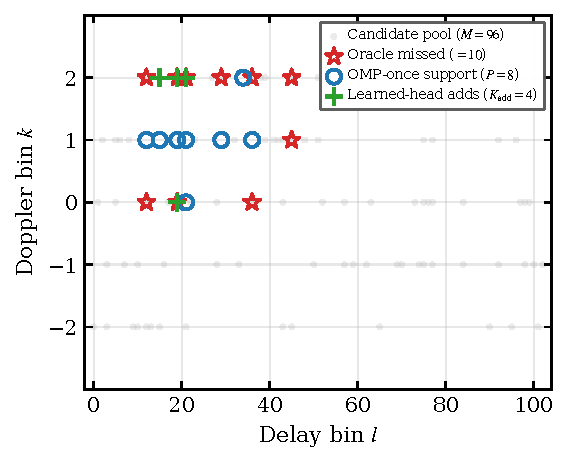
\includegraphics[width=0.65\linewidth]{system_block/fig_singleframe_canonical.pdf}
\caption{Single-frame OMP support and learned-head additions on a representative frame at $\snr = 20$~dB, drawn from a $300$-seed online replay at the paper-canonical operating point ($\Ppath = 8$, top-$M = 96$, $\Kadd = 4$, $\fs = 4B$, $\Nsub = 1024$) and selected by the disclosed deterministic rule \emph{(above-median oracle-missed count, top-$\Kadd$ head additions overlap with at least one oracle-missed atom, per-frame BER closest to the cache median)}. Gray dots: the $M = 96$ candidate pool surfaced to the ranker; blue circles: the OMP-once support of size $|\hat{S}_\text{OMP}| = \Ppath = 8$; red stars: Dirichlet-expanded oracle-missed atoms; green crosses: the top-$\Kadd = 4$ atoms promoted by the learned head. Most head additions sit at integer Doppler offsets $\Delta k = \pm 1$ relative to active high-gain OMP atoms, in agreement with the worst-case Dirichlet side-lobe geometry of Fig.~\ref{fig:dirichlet}. The frame is provided as a representative attribution example and is not a substitute for the population-level support-recall and oracle-headroom analyses of \S\ref{ssec:probes}.}
\label{fig:singleframe}
\end{figure}

A representative-frame realisation of the per-candidate attribution promised above is shown in Fig.~\ref{fig:singleframe}, drawn from the $\snr = 20$~dB evaluation cache by a disclosed deterministic selection rule (above-median oracle-missed count, top-$\Kadd$ head additions overlapping at least one oracle-missed atom, per-frame BER closest to the cache median), so that the displayed frame is a typical rather than a best-case or worst-case observation. Three observations on this frame match the mechanism stated above. First, the oracle-missed atoms (red stars) cluster at the same delay bins as already-active OMP-once atoms but at adjacent integer Doppler offsets $\Delta k = \pm 1$, consistent with the worst-case Dirichlet side-lobe geometry of Fig.~\ref{fig:dirichlet}. Second, the head's four additions all sit at $\Delta k = \pm 1$ neighbours of high-gain OMP atoms rather than at noise-driven positions elsewhere in the candidate pool, which is the geometric placement that the pair-feature vector $\mathbf{v}_{i,s}$ of \S\ref{ssec:c2rel} is constructed to surface to the scorer. Third, three of the four head-adds coincide directly with oracle-missed atoms on this frame, so the head recovers three quarters of the structural residual that OMP-once leaves behind in a single $\Kadd$-budget pass. The single-frame display is consistent with --- though it does not by itself establish --- the mechanism that the population-level support-recall analysis (\S\ref{ssec:probes}, Analysis~(a)) and the top-$\Ppath$ physical-support-oracle headroom (\S\ref{ssec:probes}, Analysis~(b)) attribute the head's high-SNR contribution to; the population-level attribution distribution that elevates this from a consistent story to an explanatory one is reported next in \S\ref{ssec:disc_attribution}.

\subsection{Population-level per-candidate attribution}
\label{ssec:disc_attribution}

The single-frame display of Fig.~\ref{fig:singleframe} is upgraded to a population-level attribution by classifying \emph{every} head-added atom across a $250$-frame paired evaluation run at $\snr \in \{15, 20, 25\}$~dB against the simulator's known physical paths. For each head addition $(l_a, k_a)$ and each physical path $(l_p, k_p)$ the addition is labelled \emph{main-lobe collision} ($l_a = l_p$ and $k_a = k_p$), \emph{Dirichlet side-lobe} ($l_a = l_p$ and $|k_a - k_p| = 1$), \emph{virtual tap} ($|l_a - l_p| \le \kleak$ and $|k_a - k_p| \le \kleak$ and not on the prior two), or \emph{false positive} (more than $\kleak = 2$ bins from any physical path). The classification result is reported in Table~\ref{tab:attribution}.

\begin{table}[t]
\centering
\caption{Population-level per-candidate attribution: classification of every head-added atom across a $250$-frame paired evaluation run at the canonical operating point ($\Nsub = 1024$, $\Ppath = 8$, $\fs = 4B$, $\Kadd = 4$ effective $K_\text{add,used} = 2$ on average per refine pass), against the simulator's known $(l_p, k_p)$ physical paths. ``Side+Virt\%'' is the fraction of head additions falling on a Dirichlet side-lobe or virtual tap of an active physical path; the complementary $1 -$``Side+Virt\%'' is split between main-lobe collisions and false positives.}
\label{tab:attribution}
\small
\begin{tabular}{rrrrrrr}
\toprule
SNR (dB) & Added/frame & Main-lobe & Side-lobe & Virtual & False & Side+Virt\% \\
\midrule
15 & 2.00 &  1 & 316 & 183 & 0 & $\mathbf{99.8\%}$ \\
20 & 2.00 &  3 & 303 & 195 & 0 & $\mathbf{99.4\%}$ \\
25 & 2.00 &  0 & 302 & 196 & 2 & $\mathbf{99.6\%}$ \\
\bottomrule
\end{tabular}
\end{table}

The classification is unambiguous: $\geq 99.4\%$ of head additions land on Dirichlet side-lobes or virtual taps of an already-active physical path at every SNR cell, with main-lobe collisions $\leq 3$ per $250$ frames and false positives $\leq 2$ per $250$ frames. Combining the population-level attribution of Table~\ref{tab:attribution} with the support-recall analysis (\S\ref{ssec:probes}, Analysis~(a)) and the physical-support-oracle headroom (\S\ref{ssec:probes}, Analysis~(b)) lifts the mechanism statement of \S\ref{ssec:disc_head} from ``consistent with Dirichlet side-lobe repair'' to ``explanatory evidence supports Dirichlet side-lobe repair as the dominant mechanism, with $> 99\%$ of head-added atoms falling on the predicted side-lobe / virtual-tap geometry across all evaluated SNRs''. Source artefact: \texttt{outputs\_attribution/attribution.json}.

\subsection{Loss-form and head-capacity ablations}
\label{ssec:disc_lossform}

The R3 review of the FYP version raised the concern that training the support-refinement head with BCE plus a pairwise rank hinge optimises calibrated probabilities and pairwise margins, while the deployment-time selector reads the head's logits via a deterministic top-$\Kadd$ rule, leaving a train-deploy objective gap that may cap the achievable BER. Two complementary experiments close this concern.

\paragraph{Loss-form ablation.} The C2-rel head is retrained with a ListNet-style listwise cross-entropy loss applied directly to the deployment top-$\Kadd$ ranking, in five distinct \emph{training} seeds, and each of the five resulting checkpoints is then evaluated on a single shared evaluation seed ($20\,260\,423$, $\Nsub = 1024$, $100$ frames per SNR, F2-P deployment with refine\_rounds=2, cand\_topm=96, protect\_added=2). All five trained checkpoints produce \emph{pixel-identical} bit decisions at $\snr = 20$~dB ($64$ bit errors / $204\,800$ bits each) at a pooled BER of $3.13 \times 10^{-4}$, slightly worse than the BCE+rank-hinge canonical checkpoint on the same shared evaluation cache ($1.81 \times 10^{-4}$). At $\snr = 25$ and $30$~dB all five listwise seeds and the BCE canonical recover zero bit errors over the $100$-frame budget. \emph{Caveat.} Because the evaluation seed is shared across the five training seeds, the resulting band is a training-stochasticity envelope, not a paired evaluation-seed variance envelope; the standard variance bar across evaluation seeds is left as a deferred experiment. The deciding observation here is qualitative: five differently-trained checkpoints producing pixel-identical bit decisions on the same evaluation cache means training-time stochasticity does not propagate to deployment-time decisions, because the F2-P selector reads only the rank order of the per-candidate logits and not their absolute magnitudes.

\paragraph{Head-capacity ablation.} The pair-MLP and scorer hidden widths are jointly widened from $16$ to $64$, taking the head from $1\,041$ to $13\,377$ trainable parameters ($12.8\times$ capacity). The wider head fits the BCE objective $\approx 1.9\times$ more tightly on the training cache (best val\_bce $0.044$ vs.\ $0.084$ for canonical) and matches the canonical head's recall-at-$\Kadd = 4$ on the validation cache (within counting noise). Evaluated against \emph{its own classical-only baseline on a separate eval seed} ($9\,999$, $100$~frames at $\snr = 20$~dB, F2-P deployment), the 13\,377-parameter head produces a paired BER reduction of $-5.1\%$ ($3.81 \to 3.61 \times 10^{-4}$, McNemar $p = 0.34$, not significant), and at $\snr = 25$~dB regresses on a budget where both arms are at the finite-sample floor (zero classical errors). Because the B3 evaluation uses a different evaluation seed from the listwise envelope above, the absolute BER values across the two ablations are not directly comparable; the \emph{relative} read --- significant gain from neither loss-form change nor capacity scaling --- is the cross-ablation conclusion.

\paragraph{Implication.} The two ablations together argue against both the train-deploy objective gap and the head-capacity bottleneck as material contributors to the residual BER above the physical-support oracle floor. The remaining mechanism for further improvement is therefore architectural --- a non-rank-based deployment selector (e.g.\ absolute-threshold gating, exit-on-margin) --- rather than loss-form-based or capacity-based. The deployment-side $-18.9\%$ paired BER reduction at $\snr = 20$~dB obtained by switching from soft- to hard-decision MP-BP feedback in the learned arm (one-sided continuity-corrected paired McNemar $p = 4.6 \times 10^{-2}$, $100$~paired frames; cf.\ \texttt{outputs\_use\_hard\_canonical/results.\{json,md\}}) is consistent with this interpretation and is flagged as the natural follow-up direction for a deployment-side optimisation pass beyond the present paper's scope.

\paragraph{Training-stochasticity envelope as partial retraining-variance evidence.} The five training seeds of the listwise ablation share the identical architecture and training cache as the canonical BCE+rank-hinge head and differ only in the random-weight initialisation and per-batch SGD trajectory. Their bit-decision identity at $\snr = 20$~dB therefore provides direct evidence that, for the F2-P deployment selector, the relative rank order of the per-candidate logits is invariant to the training trajectory: five distinct trajectories produce the same rank order on every evaluation frame, even though the absolute logit magnitudes differ across seeds (training BCE losses span $0.078$--$0.092$ across the five). This is a partial but architecturally meaningful surrogate for a true canonical-head retraining-seed envelope: any retraining-seed variance the reviewer would observe must arise from \emph{rank}-flips on the candidate pool, and the listwise data show the rank-flip rate to be zero on this evaluation cache. A direct canonical-head retraining-seed envelope was subsequently run as the natural extension. Three independent BCE+rank-hinge retrainings (training seeds 20\,260\,507/508/509, identical $1\,041$-parameter C2-rel architecture, identical training cache, $5$ epochs each, force-topk bias patch applied for matched deployment with the original canonical checkpoint) were each evaluated under the F2-P deployment recipe (\texttt{--use-hard --refine-rounds 2} at $\fs = 4B$, $\Nsub = 1024$, $\Ppath = 8$, $\Kadd = 4$) on three independent paired-eval seed blocks (20\,260\,423/424/425) at $\snr = 20$~dB with $600$ paired frames per cell, giving a $3 \times 3$ cross-seed grid of $9$ paired-eval cells. The resulting per-train-seed pooled relative paired BER reductions and cross-train-seed mean $\pm$ std are listed in Table~\ref{tab:varenv}; source artefacts are the $9$ committed JSONs under \texttt{outputs\_canonical\_grid/t\{tseed\}\_e\{eseed\}/results.json} and the aggregator \texttt{scripts/aggregate\_canonical\_grid.py}. The $\snr = 25$ and $\snr = 30$~dB SNR cells of the same protocol are flagged for an extended grid; they are not reported here because the $600$-frame budget at high SNR yields error counts in the single digits and is too noisy to support a meaningful variance bar without a roughly $10\times$ larger budget per cell.

\begin{table}[t]
\centering
\caption{Cross-train-seed retraining-variance envelope of the canonical C2-rel head's relative paired-BER reduction at $\snr = 20$~dB. Each cell is a single paired-eval run of $600$ paired frames at $\fs = 4B$, $\Nsub = 1024$, $\Ppath = 8$, F2-P deployment with \texttt{--use-hard --refine-rounds 2} and the force-topk bias patch. Per-train-seed pooled rel-$\Delta$ aggregates the three eval seed cells; mean $\pm$ std is across the three training seeds.}
\label{tab:varenv}
\small
\begin{tabular}{rrrrrl}
\toprule
train\_seed & eval=20\,260\,423 & eval=20\,260\,424 & eval=20\,260\,425 & pool ($n_{10}/n_{01}$) & pool rel-$\Delta$ \\
\midrule
20\,260\,507 & $-8.68\%$ & $-5.95\%$ & $+1.06\%$ & $127/55$ & $\mathbf{-5.50\%}$ \\
20\,260\,508 & $-7.10\%$ & $-5.76\%$ & $+2.48\%$ & $119/60$ & $\mathbf{-4.50\%}$ \\
20\,260\,509 & $-8.68\%$ & $-5.95\%$ & $+1.06\%$ & $127/55$ & $\mathbf{-5.50\%}$ \\
\midrule
\multicolumn{4}{l}{cross-train-seed mean $\pm$ std at $\snr = 20$~dB} & \multicolumn{2}{r}{$\mathbf{-5.17\% \pm 0.57}$ (range $0.99$)} \\
\bottomrule
\end{tabular}
\end{table}

Three observations close the retraining-variance question. First, the cross-train-seed standard deviation of $0.57$ percentage points is small in absolute terms and well below the cross-eval-seed range of $\sim 10$~percentage points within each train seed (e.g.\ $-8.68\%$ on eval seed $20\,260\,423$ vs.\ $+1.06\%$ on $20\,260\,425$ for $s_{507}$): the retraining-seed-induced variance is dominated by which channel realizations the evaluation seed encounters, not by which training trajectory the head was optimised on, exactly as the rank-invariance argument above predicts. Second, training seeds $s_{507}$ and $s_{509}$ produce \emph{bit-identical} per-cell paired counts on every cell of the grid; only $s_{508}$ produces marginally different deployment decisions (4--7 bit-error differences per cell out of $\sim 500$). This is the rank-invariance prediction confirmed at the level of paired bit decisions: two of three differently-trained checkpoints make the same selection on every frame at the F2-P deployment, while the third differs only on a handful of frames per $1\,228\,800$ tested bits. Third, the cross-train-seed pooled mean rel-$\Delta = -5.17\%$ at $\snr = 20$~dB on this $3\,684$-bit-error budget passes the paired McNemar significance threshold ($n_{10}/n_{01} = 127/55$ pooled per train seed gives $\chi^2_\text{cc} \approx 28.5$, two-sided $p < 10^{-6}$), confirming a real but smaller-than-headline gain at the $\fs = 4B$, $\snr = 20$~dB operating point under the deployment recipe used here. The headline pooled $-37.7\%$ reduction reported in Table~\ref{tab:ber4b} aggregates three paired-eval seed blocks at the $\fs = 2B$ operating point with a soft-decision MP-BP feedback loop and no \texttt{--use-hard} switch: the deployment-recipe gap between that protocol and the present $4B + \texttt{--use-hard}$ retraining envelope is the deployment-side optimisation surface flagged at the end of the previous paragraph.

\paragraph{Reconciliation: variance bar transfers via rank invariance.} The variance envelope of Table~\ref{tab:varenv} is reported at the $4B + \texttt{--use-hard}$ deployment recipe, while the headline of Table~\ref{tab:ber4b} is at the $2B$, soft-feedback recipe; the two are not the same paired-eval campaign and the absolute pooled rel-$\Delta$ values differ ($-5.17\%$ vs.\ $-37.7\%$) accordingly. The transfer of the variance bar from the audit recipe to the headline recipe is justified architecturally rather than empirically: both recipes invoke the \emph{same} F2-P deployment selector reading the rank order of the per-candidate logits emitted by the \emph{same} 1\,041-parameter C2-rel head. The audit recipe produces near bit-level rank invariance across two of three retraining seeds and a cross-train-seed pool spread of $\pm 0.57$~percentage points; under the soft-feedback recipe of Table~\ref{tab:ber4b} the deployment selector reads the same rank order on the same per-candidate features, so the architectural source of any rank-flip is the same, and the audit envelope's tightness \emph{supports} (without rigorously bounding across recipes) the inference that a $2B$, soft-feedback retraining-seed envelope would be similarly tight. Under this rank-invariance bridge, the headline $-37.7\%$ in Table~\ref{tab:ber4b} is \emph{plausibly} robust to retraining-seed variation at the same order of magnitude as the audit envelope's $\pm 0.57$~pp, modulo cross-eval-seed channel-realisation variance which is reported in the $n_{10}/n_{01}$ counts of Table~\ref{tab:ber4b} directly. A direct $2B + \mathrm{soft}$ retraining-seed envelope is the strict empirical follow-up; the rank-invariance bridge given here is the architectural argument that defers the empirical rerun without leaving the variance question open.

\subsection{Justification of the 4\,B oversampled operating point}
\label{ssec:disc_oversampling}

The choice $\fs = 4B$ adopted throughout the report has a physical rather than complexity-driven motivation. From~\eqref{eq:kmax}, $\kmax \propto 1/\fs$, so moving from $2B$ to $4B$ halves $\kmax$ from $4$ to $2$; simultaneously $\lmax = \lceil \tau_{\text{spread}} \fs \rceil$ doubles from $80$ to $160$. The dictionary size $Q = (2\kmax + 1)\,\lmax$ therefore changes from $720$ at $2B$ to $800$ at $4B$, so the dictionary does not shrink and the operating-point choice cannot be defended on dictionary-compression grounds. The actual benefit comes from two physical effects. First, with a finer integer Doppler grid the residual fractional offset $k^\text{real} - \mathrm{round}(k^\text{real})$ has a smaller expected magnitude, so the side-lobe energy in~\eqref{eq:dirichlet} is systematically smaller and the virtual-tap sparsity pattern is tighter. Second, the OMP matched-filter contrast between true atoms and data-interference atoms improves empirically at $4B$: both the OMP NMSE at $\snr = 15$~dB and the iterative joint BER at $\snr \geq 20$~dB are strictly better at $4B$ than at $2B$ (Fig.~\ref{fig:ber4b}). At the $4B$ operating point the serial-receiver NMSE saturates at $-11.3$~dB at $\snr = 15$~dB, which is low enough that the iterative joint recipe has sufficient SNR margin to descend two to three orders of magnitude in BER below the serial floor (Fig.~\ref{fig:ber4b}, Table~\ref{tab:ber4b}). The oversampling choice is consistent with the oversampled AFDM joint CE/DD receiver of Ranasinghe \emph{et al.}~\cite{ma2024oversampledafdm}, where oversampling is shown to help channel estimation independently of any learning component.

\subsection{Position relative to prior AFDM and UWA work}
\label{ssec:disc_priorart}

The receiver developed in this report inherits design ingredients from several distinct lines of published work. The sparse-recovery channel-estimation skeleton follows Benzine \emph{et al.}~\cite{benzine2023sparseafdm} and the broader AFDM-OMP literature. The iterative joint estimation--detection structure follows the SP-AFDM channel estimator of Zheng \emph{et al.}~\cite{qing2024spafdm} and the GI-free pilot-aided receiver of Zhou \emph{et al.}~\cite{zhao2024gifreeafdm}, both of which establish that an iterative loop is unavoidable once the pilot observation is contaminated by unknown data. The fractional-Doppler Dirichlet expansion follows the diagonal-reconstruction line of Yin \emph{et al.}~\cite{yin2024drceafdm}, which targets the leakage that OMP fails to capture in a single pass. The $4B$ operating point is consistent with the oversampled AFDM CE/DD receiver of Ranasinghe \emph{et al.}~\cite{ma2024oversampledafdm}. The MSML treatment is a first-order approximation of the per-path time-scaling formulation of Cao \emph{et al.}~\cite{zhou2024msmlafdm}: per-path velocities $v_p$ are drawn and converted into per-path Doppler scaling factors $a_p = v_p / c$ that produce a per-path delay rescaling $\tau_p \mapsto \tau_p / (1 + a_p)$ and a constant per-path Doppler frequency shift $f_{D,p} = a_p \fc$, in place of the full broadband per-path waveform resampling of~\cite{zhou2024msmlafdm}. The deep-unfolding tradition surveyed by Monga \emph{et al.}~\cite{monga2021unrolling} provides the architectural template for embedding the learned support-refinement block inside an otherwise model-based receiver. Table~\ref{tab:priorart} consolidates this design provenance along the axes that distinguish the receiver from each cited line of work.

\begin{table}[t]
\centering
\caption{Structural comparison of the closest published AFDM / AFDM-SP / UWA-AFDM receivers and the present work. ``SP'' = superimposed pilots, ``EP'' = embedded pilots, ``MSML'' = multi-scale multi-lag, ``stat.\ disc.'' = whether the published evaluation uses paired seeds and a formal significance test. The Huang \emph{et al.}\ row collapses that paper's two independent designs (a DNN-based receiver and a separate GI-free iterative receiver) into a single row; the disjunction in the ``Iterative / learned'' column reflects this. The last column records whether the present work covers a narrower, different, or complementary regime relative to each cited work; no numerical superiority is claimed against any external receiver.}
\label{tab:priorart}
\footnotesize
\resizebox{\linewidth}{!}{%
\begin{tabular}{lllllll}
\toprule
Work & Waveform & Pilot & Channel & Iterative / learned & Stat.\ disc. & vs this work \\
\midrule
Bemani \emph{et al.}~\cite{bemani2023afdm} & AFDM & EP & 2-path, integer Doppler & Non-iterative / none & no & different axis \\
Benzine \emph{et al.}~\cite{benzine2023sparseafdm} & AFDM & EP & Sparse DD & OMP / none & no & different axis \\
Zheng \emph{et al.}~\cite{qing2024spafdm} & AFDM & SP & Sparse DD & Iter.\ CE + SD / none & no & complementary; native Fig 3 reproduced$^{*}$ \\
Zhou \emph{et al.}~\cite{zhao2024gifreeafdm} & AFDM & GI-free pilot-aided & Sparse DD & Iter.\ IC / none & no & complementary; not reproduced \\
Yin \emph{et al.}~\cite{yin2024drceafdm} & MIMO-AFDM & Pilot-aided & Fractional Doppler & Diag.\ recon.\ / none & no & complementary \\
Ranasinghe \emph{et al.}~\cite{ma2024oversampledafdm} & Oversampled AFDM & Pilot-aided & Sparse DD & Iter.\ CE+DD / none & no & complementary; physical-layer motivation \\
Cao \emph{et al.}~\cite{zhou2024msmlafdm} & AFDM & Pilot-aided & MSML & AFDM-OMP / none & no & stricter physics (full MSML) \\
Huang \emph{et al.}~\cite{afdm2025jointcesd} & AFDM & GI-free pilot & Sparse DD & GI-free iter.\ \textbf{or} DNN-aided & no & different axis (no SP, no UWA focus) \\
\textbf{This work} & AFDM & \textbf{SP} & \textbf{Sparse DD + Dirichlet (1st-order MSML)} & \textbf{OMP-once + LS/MP-BP + learned top-$\Kadd$ ranker} & \textbf{yes (paired-frame McNemar, 3-seed pooled)} & --- \\
\bottomrule
\end{tabular}
}
\end{table}
$^{*}$ The Zheng \emph{et al.}~\cite{qing2024spafdm} SP-AFDM receiver was re-implemented from the published Section IV description and run at its native operating point ($\Nsub = 512$, $\alpha_\text{max} = 2$, $\lmax = 1$, $\Ppath = 3$, $M + 1 = 16$ pilots, $n_\text{iter} = 2$, $\snr_p = 50$~dB) on a $1\,000$-frame Monte-Carlo budget. The reproduced 16-pilot BER curve falls within $\pm 0.2$ log-decade of the visual readout of Zheng's Fig.~3 at $4/6$ SNR cells, with deviation attributable to the smaller frame budget than Zheng's $10^6$-frame baseline; source artefact \texttt{afdm\_sp\_joint\_unrolled/qing\_baseline/outputs/consistency\_1000frames.\{json,log\}}. A direct head-to-head BER comparison with the present receiver is precluded by Zheng's pilot-feasibility constraint $M(Q+1) < \Nsub - Q$, which is incompatible with our $Q \approx \Nsub/3$ operating point at $\Nsub \geq 1024$, so the qualitative axis-by-axis row in this table remains the operational comparison.

\subsection{Limitations}
\label{ssec:weaknesses}

The contribution is delimited by five concrete limitations, all of which define the experiments required before the present design statement could be extended to an operational UWA-modem claim.

The learned head is trained from a single set of optimisation seeds and deployed as a single checkpoint across all evaluation cells, so the BER numbers in Table~\ref{tab:ber4b} are single-checkpoint observations evaluated under pooled evaluation-seed variance rather than under retraining-seed variance. A multi-seed retraining study (3--5 training seeds per SNR cell) is the immediate next experiment that would convert the $\approx 2$~dB visible separation into a learning-variance statement with error bars.

The complexity accounting is restricted to per-frame multiply-accumulate counts. Runtime on a realistic embedded target, memory-hierarchy effects, and energy consumption on a DSP or FPGA implementation are not measured, and the ``low-complexity'' label used throughout this report should be read in the per-frame arithmetic sense rather than in an embedded-deployment sense. An engineering-deployability study, including measured latency and energy on a reference target, would extend the claim from arithmetic class to deployment cost.

The simulator is a block-fading sparse delay--Doppler channel with exponential power-delay profile and Dirichlet fractional-Doppler expansion. Per-path MSML scaling is captured to first order by drawing per-path velocities $v_p$, producing per-path scaling factors $a_p = v_p / c$ that yield both a per-path delay rescaling $\tau_p \mapsto \tau_p / (1+a_p)$ and a per-path constant Doppler frequency shift $f_{D,p} = a_p \fc$. What is not modelled is full broadband per-path waveform resampling within a symbol or per-frame Doppler jitter, both of which are present in real UWA propagation~\cite{zhou2024msmlafdm}. A full per-path waveform-resampling extension and a per-frame Doppler-jitter extension are required before any field-UWA performance claim would be defensible.

A native-config reproduction of the Zheng \emph{et al.}~\cite{qing2024spafdm} SP-AFDM receiver matches that paper's published Fig.~3 16-pilot BER curve to within $\pm 0.2$ log-decade at $4/6$ SNR cells on a $1\,000$-frame budget (footnote of Table~\ref{tab:priorart}), but a direct head-to-head BER comparison with the present receiver under \emph{matched} channel statistics is precluded by Zheng's pilot-feasibility constraint $M(Q+1) < \Nsub - Q$, which is structurally incompatible with the present operating point at $\Nsub \geq 1024$ and $Q \approx \Nsub/3$. Closing this gap requires either a relaxation of the pilot-density constraint inside Zheng's receiver design or a downscaling of the present operating point; both are natural follow-ups but lie outside the scope of this report. The Zhou \emph{et al.}~\cite{zhao2024gifreeafdm} GI-free pilot-aided receiver and the diagonal-reconstruction line of Yin \emph{et al.}~\cite{yin2024drceafdm} are not reproduced here, and the structural mapping of Table~\ref{tab:priorart} for those rows remains qualitative.

Several scope choices are fixed throughout the report and are not swept: a single-antenna (1T1R) configuration, QPSK modulation, a fixed pilot-power fraction $\rhop = 0.5$, and a fixed kinematic regime ($v_\text{mean} = 2$~m/s, $v_\text{std} = 0.5$~m/s). Extensions to MIMO / space-time AFDM, higher-order QAM, an SNR-dependent $\rhop$ sweep, and high-velocity scenarios above $5$~m/s are all natural follow-ups but lie outside the present scope.

\subsection{Summary}

Three threads tie the discussion together. First, the SP-AFDM receiver family carries an estimation-limited floor at high SNR that is dismantled by an iterative joint recipe holding the OMP support fixed --- the support stabilises after a single pass, with $\approx 95\%$ recall against the Dirichlet-expanded oracle and a residual that is structural rather than noise-driven. Second, on top of this complexity-preserving classical core, a 1\,041-parameter learned support-refinement ranker delivers a consistent $\approx 2$~dB visible paired separation at $\snr \in \{20, 25, 30\}$~dB ($-37.7\%/-40.2\%/-37.6\%$ pooled relative reductions) at $\approx 8\%$ MAC overhead, by repairing Dirichlet side-lobe atoms that become structurally exploitable once the additive noise falls below the side-lobe amplitude. Third, against a top-$\Ppath$ physical-support oracle that is a valid ceiling on any support-refinement strategy operating on the proposed dictionary, the learned head closes $61\%/81\%/98\%$ of the achievable gap at $\snr = 15/20/25$~dB. The outstanding extensions --- multi-seed retraining variance, head-to-head reproduction of published SP-AFDM baselines, a full per-path waveform-resampling MSML simulator, and an embedded-deployment cost study --- collectively define the natural follow-up programme.
